%%%%%%%%%%%%%%%%%%%%%%%%%%%%%%%%%%%%%%%%%%%%%%%%%%%%%%%%%%%%%%%%%%%%%%%%%
%% Bachelor's & Master's Thesis Template                                %%
%% Created by Artur M. Brodzki & Piotr Woźniak  (2019-2010)             %%
%% Faculty of Electronics and Information Technology                    %%
%% https://www.overleaf.com/latex/templates/wut-thesis/vfvvdqztfqbt     %%
%% Modified by Kinga Węzka (2021)                                       %%
%% Faculty Geodesy and Cartography                                      %%
%% Warsaw University of Technology                                      %%
%%%%%%%%%%%%%%%%%%%%%%%%%%%%%%%%%%%%%%%%%%%%%%%%%%%%%%%%%%%%%%%%%%%%%%%%%

\documentclass[
    left=2.5cm,         % Sadly, generic margin parameter
    right=2.5cm,        % doesnt't work, as it is
    top=2.5cm,          % superseded by more specific
    bottom=3cm,         % left...bottom parameters.
    bindingoffset=6mm,  % Optional binding offset.
    nohyphenation=false % You may turn off hyphenation, if don't like.
]{gik/gik-thesis}

\langpol 				% dla języka angielskiego: \langeng
\graphicspath{{img/}}   % ścieżka względna do katalogu z  obrazkami.

\begin{document}

%--------------------------------------
% Strona tytułowa
%--------------------------------------
\EngineerThesis % dla pracy magisterskiej: \MasterThesis, dla inzynierskiej: \EngineerThesis

\zaklad{Zakład Geodezji i Astronomii Geodezyjnej}

\kierunek{YYYYY}
\specjalnosc{YYYY} % dotyczy pracy magisterskiej
\title{
    Niepotrzebnie długi i skomplikowany tytuł pracy \\
    trudny do przeczytania, zrozumienia i wymówienia 
}
\engtitle{ % Tytuł po angielsku do angielskiego streszczenia
    Unnecessarily long and complicated thesis' title \\
    difficult to read, understand and pronounce
}
\ThesisNumber{numer pracy według wydziałowej ewidencji prac <liczba>}
%\ThesisNumber{thesis number in the Faculty thesis register <number>}

\author{\{Kinga Węzka\}}
\album{XXXXXX}

\promotor{Mikołaj Kopernik}
\konsultacje{Wincenty Długosz}
\date{\the\year}

\maketitle

%--------------------------------------
% Streszczenie po polsku
%--------------------------------------
\cleardoublepage % Zaczynamy od nieparzystej strony
\streszczenie
Here goes abstract


\slowakluczowe XXX, XXX, XXX   
\abstract 
Here abstract content

\keywords XXX, XXX, XXX

ljngisjng ksjbdflakbkbsvksda  

%--------------------------------------
% Oświadczenie o autorstwie
%--------------------------------------
\cleardoublepage  % Zaczynamy od nieparzystej strony
\pagestyle{plain}
\makeauthorship

%--------------------------------------
% Spis treści
%--------------------------------------
\cleardoublepage % Zaczynamy od nieparzystej strony
\tableofcontents

%--------------------------------------
% Rozdziały
%--------------------------------------
\cleardoublepage % Zaczynamy od nieparzystej strony
\pagestyle{headings}
% Wygodnie jest trzymać każdy rozdział w osobnym pliku.
% Umożliwia to również łatwą migrację do nowej wersji szablonu
% wystarczy podmienić swoje pliki.
% Wszystckie pliki tex z rozdziałami znajdują się w folderze "content"
\newpage % Rozdziały zaczynamy od nowej strony.
\section{Wstęp}

Obrazkiem zamiast tekstu o składzie edytorskim prac dyplomowych ;):
\cite{Wezka2021}



\begin{figure}[!ht]
	\centering 
\includegraphics[width=0.55\textwidth]{formatowanie_pracy_dyplomowej.jpg}
	\caption{Title}\label{fig:1}
\end{figure}

\subsection{Podrozdział}
dodanie treści
\subsubsection{Podpodrozdział}
W plikach OneDrive przedmiotu  (\url{informatyka4gik/IT_GIK_LaTeX}) znajduje się templatka pracy dyplomowej (\url{WUT-GIK_Thesis.zip}) opracowana w języku LaTeX. 
Wzór przygotowany został zgodnie z wytycznymi pisania prac dyplomowch w Politechnice Warszawskiej.
Do uruchomienia i edycji dokumentu potrzebna jest dystrybucja systemu LaTeX (kompilator języka) oraz wybrany edytor IDE (np. TeXStudio): 
\begin{itemize}
    \item MIK\TeX{} dystrybucja systemu LaTeX: \url{https://miktex.org/download}
    \item \TeX Studio edytor IDE: \url{https://www.texstudio.org}
\end{itemize}

\begin{itemize}
    \item \TeX{} -- jest systemem składu dokumentów i książek, powstałym pierwotnie na potrzeby prac naukowych z nauk ścisłych. Program powstał w Stanach Zjednoczonych na Uniwersytecie Stanforda. Jego twórcą jest \textbf{Donald E. Knuth}, amerykański matematyk i informatyk.
    Pierwsza wersja pojawiła się publicznie już w 1978 roku, jendak dopiero w 1989 r. system ten, nazwany \TeX, został uznany za ukończony.
    Kolejne wersje numerowane sa w oparciu o rozwinięcie dzięsiętne liczby $\pi$. W grudniu 2014 roku \TeX doczekał się numeru 3.14159265.
    \item \LaTeX{} -- jest zestawem skryptów i makt systemy \TeX{}, przez co jest bardziej przyjazny dla użytkownika. Opracowany przez \textbf{Leslie Lamport}. Obecna wersja \LaTeX{} to \LaTeX{} 2$\epsilon$
\end{itemize}


System składu oparty na programie \LaTeX{}, przygotowany na określoną platformę systemową, nazywamy dystrybucją. Najbardziej popularne dystrybucje \LaTeX{} to:
\begin{itemize}
    \item MIK\TeX: \url{www.miktex.org/}, dystrybucja systemu {\TeX} dla systemów Windows, Linux i macOS -- polecany dla Windows \\
    \item \TeX Live: \url{www.tug.org/texlive/}, dystrybucja systemu {\TeX} dla systemów Windows, Linux i macOS -- polecany ndla linux\\
\end{itemize}


\textbf{Wybrane kompilatory \LaTeX{}:}, na podstawie \citep{Borkowski.Przybylski2015}
\begin{itemize}
    \item \TeX -- podstawowy silnik umożliwiający kompilowanie plików źródłowych \TeX. Generuje pliki w formacie DVI, który ustąpił już miejsca innym, popularniejszym formatom (np. pdf). Ten i inne powody sprawiły, że jest obecnie używany bardzo rzadko.
    \item e-\TeX -- rozszerzenie \TeX o nowe polecenia ułatwiające pisanie makr. Zastosowane w nim ulepszenia zostały zaimplementowane w innych, nowszych silnikach
    \item pdf\TeX -- oparty został na silniku e-\TeX, ale rozszerza go o możliwości związane z generowaniem plików PDF. Tym samym pdfTeX może generować zarówno pliki DVI, jak i PDF. Jest to obecnie najpopularniejszy z używanych silników.
    \item Xe\TeX -- został oparty na kompilatorze e-\TeX, ale wspiera natywnie kodowanie UTF-8 oraz umożliwia dostęp do fontów (krojów pisma) zainstalowanych w systemie operacyjnym, również takich jak OpenType oraz AAT. 
    \item Lua\TeX -- nazywany początkowo drugą wersją pdf\TeX, wspiera natywnie kodowanie UTF-8, ale też umożliwia wykorzystywanie w pracy języka programowania o nazwie Lua, dzięki któremu można (między innymi) uzyskać dostęp do fontów systemowych. Opiera się na silniku pdfTeX.
\end{itemize}


\newpage
\subsection{Struktura plików dla templatki pracy dyplomowej WUT-GIK-Thesis}

\begin{verbatim}
└── <WUT-GIK-Thesis>
    ├── <content>
    │   ├── 1-wstep.tex
    │   ├── 1.1-formatowanie_tekstu.tex
    │   ├── 1.2-cytowania.tex
    │   ├── 1.3-wypunktowania.tex
    │   ├── 2-wzory.tex
    │   ├── 2.1-rysunki.tex
    │   ├── 2.1-tabele.tex
    │   ├── 2.3-wstawianie_kodu.tex
    │   ├── 4-podsumowanie.tex
    │   ├── appendix1.tex
    │   └── appendix2.tex
    ├── <gik>
    │   ├── gik-thesis.cls
    │   ├── header-eng.png
    │   ├── header.png
    │   ├── oswiadczenie_autora_pracy.pdf
    │   ├── thesis_author_declaration-1.pdf
    │   ├── thesis_author_declaration-1.pdf
    │   ├── title-inz-eng.png
    │   ├── title-inz.png
    │   ├── gik-thesis.cls
    │   ├── title-mgr-eng.png
    │   └── title-mgr.png
    ├── <img>
    │   ├── machine_learning.jpg
    │   ├── od_polinistow.png
    │   ├── poziom_istotnosci.jpg
    │   └── itd.jpg
    ├── bibliografia.bib 
    ├── buildPres
    ├── main.tex     (plik z polskimi opisami)
    ├── main.pdf     (skompilowany main_pl.tex)
    ├── main_en.tex  (main file with english comments)
	├── main_en.pdf  (compiled main_en.tex)
    └── wprowadzenie_latex_prezentacja.pdf 
\end{verbatim}

\newpage
\subsection{Podstawowa struktura dokumentu}
 Podstawowa struktora dokumentu składa się z 3 etapów:
 \begin{enumerate}
    \item KLASA DOKUMENTU -- zdefiniowanie klasy dokumentu (np.books, article, report, letter lub klasa własna) oraz podstawowych opcji.
    \item PREAMBUŁA -- ustawień ogólne całego dokumentu (np. pakiety, makra etc.)
    \item TREŚĆ DOKUMENTU -- cała treśc dokumentu (rozdziały, sekcje, wzory etc.)
 \end{enumerate}

\begin{lstlisting}[language=tex,caption={\emph{Podstawowa struktura dokumentu TeX} }]
% --- 1. KLASA DOKUMENTU
\documentclass[options]{class}

% --- 2. PREAMBUŁA
\usepackage{polski}         % jez. polski, znaki diakrytyczne
\usepackage[utf8]{inputenc} % system kodowania tekstu

% --- 3. TREŚĆ DOKUMENTU
\begin{document}
	
Tutaj znajduje się cała treść dokumentu, 
rozdziały, podrozdziały etc. tak jak zostało opisane w 

\end{document}
\end{lstlisting}


Tutaj będzie cytowanie \citep{Wanninger1993}
        
\subsection{Formatowanie tekstu} 

\begin{itemize}
\item Automatyczne łamanie liniii stron, akapity oddzielane są od siebie pustymi liniami. Ilość użytych spacji i/lub pustych linii nie ma znaczenia.
\item "myślniki"
\begin{itemize}
    \item - dywiz (hyphen): \verb|-|
    \item -- łącznik (short dash): \verb|--|
    \item --- myślnik (long dash): \verb|---|
\end{itemize}
\item Rodzaj i grubość czcionki:
\begin{itemize}
    \item \verb|\textrm{tekst}| - \textrm{tekst} – pismo proste,
    \item \verb|\textsl{tekst}| - \textsl{tekst} – pismo proste pochylone
    \item \verb|\textit{tekst}| - \textit{tekst} – kursywa (italic),
    \item \verb|\emph{tekst}|   - \emph{tekst}    – wyróżnienie (zalecane),
    \item \verb|\textbf{tekst}| - \textbf{tekst} – pismo pogrubione (bold),
    \item \verb|\texttt{tekst}| - \texttt{tekst} – pismo imitujące pismo maszynowe
    \item \verb|\textsf{tekst}| - \textsf{tekst} – pismo bezszeryfowe
\end{itemize}
\item Wielkość czcionki definujemy w opcjach klasy dukumentu, czyli:
\begin{verbatim}
\documentclass[10pt,a4paper]{article}
\end{verbatim}
\item Nastepnie wielkość czcionki w stosunku do \emph{normalsize} zieniamy poprzez:
\begin{verbatim}
\tiny           % 5pt
\scriptsize     % 7pt
\footnotesize   % 8pt
\small          % 9pt
\normalsize     % 10pt
\large          % 12pt
\Large          % 14pt
\LARGE          % 17pt
\huge           % 20pt
\Huge           % 25pt
\end{verbatim}
\end{itemize}
 
\subsection{Cytowania}
Za tworzenie bibliografi w \LaTeX{} odpowiedzialny jest Bib\TeX{} narzędzie służące do formatowania bibliografii według zadanych kryteriów. Bib\TeX{} ułatwia dostosowanie uprzednio zebranych danych bibliograficznych do wymogów różnych wydawców. W preambule dokumentu należy zaimportowac odpowiedni pakiet oraz zdefiniowac zestaw ustawień tak aby generowana bibliografia dokumentu odpowiadałam zdefiniowanym wymaganiom. W pracach dyplomowych wymaga się użycia stylu cytowania o nazwie \emph{Harvard}. Taki styl cytowania został zdefiniowany w niniejszym dokumencie.

\begin{lstlisting}[language=Python,	caption={\emph{Dokument LaTeX z bibliografią} }]
\documentclass[A4]{gik-thesis}

\RequirePackage[natbibapa]{apacite} % bibliography natbib
\bibliographystyle{apacite}
\renewcommand{\BBAA}{i} 
\renewcommand{\BBAB}{i} 
\renewcommand{\BOthers}{i in} 

\begin{document}
Treść dokumentu na podstawie \citep{Nowak.Kowalski2018}
% wygenerowanie bibliografi na końcu dokumentu
\bibliography{bibliografia} % nazwa pliku z bibliografia (plik *.bib) 
\end{document}
\end{lstlisting}


\begin{lstlisting}[language=Python,	caption={\emph{Przykładowy plik \url{bibliografia.bib} } }]
@Book{Nowak.Kowalski2018,
	author      = {Piotr Nowak and Jan Kowalski},
	title       = {Opowiadanie o niczym},
	publisher   = {PWN},
	year        = {2018},
}
\end{lstlisting}

Jak widać na obrazku numer \ref{fig:obrazekB}

Poniżej znajdują się przykłady użycia cytowania, więcej na ten temat można znależć na oficjalnej stronie biblioteki:\footnote{\url{http://merkel.texture.rocks/Latex/natbib.php}},\footnote{Odniesienia można napisać na stronie korzystając z komendy footnote{}}
Druga liczba oznacza wcięcie od prawej \citep{Hofmann-Wellenhof.etal2008} lub \citep[ch.VII]{Teunissen.Montenbruck2017}

Jeśli jest wielu Autorów podajemy imię pierwsego oraz "" \citep{Bertiger.etal2009}

\begin{lstlisting}[language=Python,	caption={Przykłady cytowań}]
\citet{jon90}	       > Jones et al. (1990)
\citet[chap. 2]{jon90} > Jones et al. (1990, chap. 2)
\citep{jon90}	       > (Jones et al., 1990)
\citep[chap. 2]{jon90} > (Jones et al., 1990, chap. 2)
\end{lstlisting}


Cytowania stron internetowych np. \citep{NCEI2020} lub \cite{ASGEUPOS2021}:
\begin{lstlisting}[language=Python,	caption={\emph{Cytowania stron internetowych n} }]
@Misc{NCEI2020,
	author       = {NCEI},
	howpublished = {\url{https://www.ngdc.noaa.gov}},
	note         = {Dostęp : 2020-09-30},
	title        = {World Magnetic Model 2020},
	year         = {2020},
	doi          = {10.25921/11v3-da71},
}
\end{lstlisting}

Kilka cytowań \citep{Teunissen.Montenbruck2017,Wanninger1993,Hofmann-Wellenhof.etal2008,NCEI2020,ASGEUPOS2021}
 

\subsection{Wypunktowania}
\subsubsection{Punktacja}

\begin{itemize}
    \item Item 1:
    \begin{itemize}
        \item item 1.1;
        \item item 1.2;
        \item item 1.3;
    \end{itemize}
    \item Item 2;
    \item Item 3;
    \item Item 4.
\end{itemize}


\subsubsection{Numeracja}
\begin{enumerate}
    \item Item 1:
    \begin{enumerate}
        \item item 1.1;
        \item item 1.2:
        \begin{enumerate}
            \item item 1.2.1;
            \item item 1.2.2;
        \end{enumerate}
        \item item 1.3;
    \end{enumerate}
    \item Item 2;
    \item Item 3;
    \item Item 4.
\end{enumerate}

 

\newpage % Rozdziały zaczynamy od nowej strony.
\section{Rodział 2}

Citation \citep{Wanninger1993}

\citet{Bertiger.etal2009}

\subsection{Mathematical expression inline}


La\TeX allows two writing modes for mathematical expressions: the inline math mode and display math mode:
\begin{itemize}
	\item \emph{inline} math mode is used to write formulas that are part of a paragraph \\
	
	In physics, the mass-energy equivalence is stated by the equation $E=mc^2$, discovered in 1905 by Albert Einstein.
	
	
	\item \emph{display} math mode is used to write expressions that are not part of a paragraph, and are therefore put on separate lines.: 
	
	In physics, the mass-energy equivalence is stated by the equation
	\begin{equation}
		E=mc^2,
	\end{equation}
	discovered in 1905 by Albert Einstein.
\end{itemize}

\url{https://en.wikibooks.org/wiki/LaTeX/Mathematics}


\subsection{Wzory}
Zestaw syymboli matematycznych znajduje się w plikach, \url{LaTeX_symbols_short.pdf}
oraz \url{LaTeX_symbols_full.pdf}, dostępnych w folderze \url{LaTeX/latex_bibliography} na dysku \href{https://wutwaw-my.sharepoint.com/:f:/g/personal/kinga_wezka_pw_edu_pl/EjJEPFmm2bFKvw8gDpzh20QBpIyHB2EN0uaUE3e4bqPH9w?e=OBLJ3e}{OneDrive}.
Dodatkowe informacje na temat wyrażeń matematycznych w La\TeX{}:
\url{http://www.latex-kurs.x25.pl/paper/wyrazenia_matematyczne}




Einstein rozwinął \emph{szczególną teorią względności} (STW), gdzie poprawnie przewidział równoważność masy i energii, fakt ten został wyrażony przez słynny wzór: 
\begin{equation}\label{eq:Einstein}
    E  = mc^2 + \frac{1}{2}  \frac{10}{100} \sigma \alpha 
\end{equation}
gdzie:
\begin{conditions*}
E & energia [\si{kg.m^2.s^{-2}}] czyli dżul [\si{\joule} ], \\
m & masa w jednostkach \si{\kilogram},    \\
c^2 & prędkość światła w próżni \si{\metre\per\second}, \\
x & którego nie ma we wzorze więc nie powinno byc wyjaśniene, tutaj służy tylko po to, aby pokazać, że bardzo długi opis zostanie odpowienio wyrównany.
\end{conditions*}

Według wzoru \ref{eq:Einstein}

\begin{table}\caption{tytuł tabeli}\label{tab:1}
	\centering
\begin{tabular}{c c c}
		\midrule
		Here & there & where \\ \midrule
		1    & 2     & 3 \\
		4 	 & 5     & 6  \\
		3	 & 4     & 6 \\\midrule
\end{tabular}
\end{table}



Kilka słów o jednostkach, najlepiej użyć do tego biblioteki \citep{Bertiger.etal2009} siunit\footnote{\url{http://mirrors.ibiblio.org/CTAN/macros/latex/contrib/siunitx/siunitx.pdf}}. Wtedy zapisując komendy:
\begin{lstlisting}[language=tex,caption={\emph{Wybrane komendy biblioteki siunit}}]
\si{kg.m.s^{-1}} \\
\si{\kilogram\metre\per\second} \\
\si[per-mode=symbol]
{\kilogram\metre\per\second} \\
\si[per-mode=symbol]
{\kilogram\metre\per\ampere\per\second}
\end{lstlisting}
otrzymamy następujące wyniki: 
\si{kg.m.s^{-1}} \\
\si{\kilogram\metre\per\second} \\
\si[per-mode=symbol]
{\kilogram\metre\per\second} \\
\si[per-mode=symbol]
{\kilogram\metre\per\ampere\per\second}



\subsection{Macierze i wzory wieloninijkowe}

\begin{equation}\label{eq:matrix1}
	\begin{bmatrix}
		\cos{\theta}    & \sin{\theta}   & 0 \\
		-\sin{\theta}   & \cos{\theta}   & 0 \\
		0              &  0             & 1 \\
	\end{bmatrix}
\end{equation}


\begin{align}\label{eq:wzor_macierz}
\begin{bmatrix}
    1 & 0 & 0 \\
    0 & 2 & 0 \\
    0 & 0 & 3
\end{bmatrix} \cdot
\begin{bmatrix}
    4 \\ 5 \\ 6
\end{bmatrix} =
\begin{bmatrix}
    4 \\ 10 \\ 18
\end{bmatrix}
\end{align}

\subsection{Podział długich równań}
Pamietajmy aby bardzo długie wzory dzielić

\begin{equation}
\begin{split}
F 	& = \{F_{x} \in  F_{c} 	: (|S| > |C|) \\
	&\quad \cap (\text{minPixels}  < |S| < \text{maxPixels}) \\
	&\quad \cap (|S_{\text{conected}}| > |S| - \epsilon) \}
\end{split}
\end{equation}
	
\begin{equation}
    \begin{split}
        x   & = \sigma + \frac{1^2}{2} N \sin{B} \cos{B} \\
        & + \frac{1^2}{12} \cos^2{B} \cdot \left( 5 - t^2 + 9 \eta^2 + 4 \eta^2 \right)  \\
        & +\frac{1^4}{360} \cos^4{B} \cdot \left( 61 \eta^2 t^2 \right) + \ldots 
    \end{split}
\end{equation}

\subsection{Równania i podrównania}
\begin{subequations}\label{eq:abc}
    \begin{align}
        X_k   &= X'_k \cos \Omega_k -  Y'_k \cos i_k \sin \Omega_k   \label{eq:a} \\
        Y_k   &= X'_k \sin \Omega_k -  Y'_k  \cos i_k \cos \Omega_k  \label{eq:b} \\
        Z_k   &= Y'_k  \sin i                                        \label{eq:c}
    \end{align}
\end{subequations}
Odniesienia do całego równania \eqref{eq:abc}, oraz do kolejnych równań \eqref{eq:a}, \eqref{eq:b}, \eqref{eq:c}


 
\newpage
\subsection{Rysunki}

\begin{figure}[!ht]
	\centering 
	
\includegraphics[width=0.5\textwidth]{od_polinistow.png}
	\caption{Pozdrowienia od polonistów}\label{fig:polonistyka}
\end{figure}

\begin{figure}[!ht]
	\centering
	\begin{subfigure}[b]{0.45\textwidth}
		\centering
		
\includegraphics[height=0.3\textheight,keepaspectratio]{poziom_istotnosci.jpg}
		\caption{Obrazek YX}\label{fig:obrazekA}
	\end{subfigure}
	~ %add desired spacing between images, e. g. ~, \quad, \qquad, \hfill etc. 
	%(or a blank line to force the subfigure onto a new line)
	\begin{subfigure}[b]{0.45\textwidth}
		\centering
		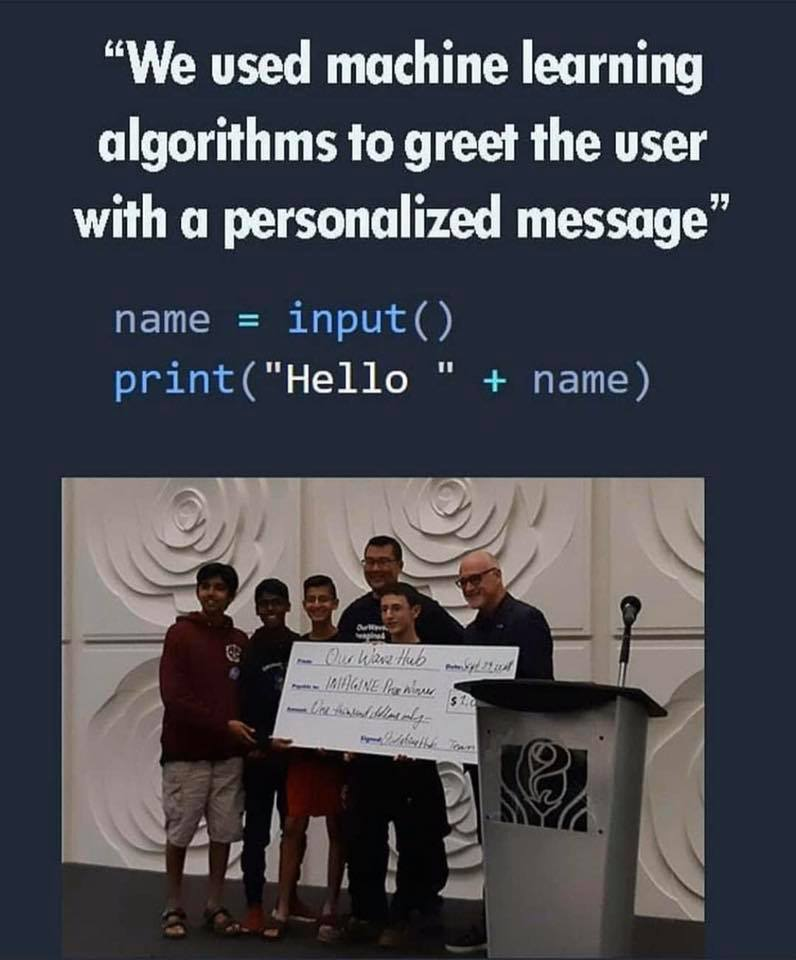
\includegraphics[height=0.3\textheight,keepaspectratio]{machine_learning.jpg}
		\caption{Obrazek XY}\label{fig:obrazekB}
	\end{subfigure}
	\caption{Dwa rysunki obok siebie}\label{fig:Obrazki}
\end{figure}

Odniesienia do rysunków np. Jak pokazano na rysunku \ref{fig:polonistyka} oraz \ref{fig:obrazekA}.
Natomiast rynunek \ref{fig:Obrazki} opisuje to samo zjawisko.




\subsection{Tabele}

Do tworzenia tabeli służy otoczenie \lstinline|tabular|, schemat tworzenia tabely przypomina tworzenie macierzey w środowisku LaTeX.
kolumy odzielamy symbolem -- ampersant), wiersze odzielamy symolem -- podwójny backslesh. Do wygenerowania kodu tabeli można wykorzystać 
generator tabel online: \url{https://www.tablesgenerator.com/}. Pozwala on definiować tabele jak również wykonac konwersję tabeli xls do kodu LaTex.

\begin{figure}[!ht]
	\centering 
	
\includegraphics[width=.33\textwidth]{od_polinistow.png}
	\caption{Co jest na rysunku}\label{fig:polonistyka}
\end{figure}



\begin{table}[!h] \label{tab:tabela1} \centering
\caption{Przykładowa tabela.}
\begin{tabular} { c  c  r }
	\toprule[1pt]
    Kolumna 1 & Kolumna 2 & Liczba  	\\ \midrule
    cell1     & cell2     & 60 		 	\\
    cell4     & cell5     & 43 		 	\\
    cell7     & cell8    & 20,45 		\\ \midrule
    \multicolumn{2}{r}{Suma:} & 123,45 \\ \bottomrule[1pt]
\end{tabular}
\end{table}

\kant[2]

\begin{longtable}{| c | m{0.58\linewidth} | r | m{0.1\linewidth} |}
    \caption{Tabela wielostronicowa.} \\
    \hline
    Lp & \multicolumn{1}{c|}{Treść} & \multicolumn{1}{c|}{Kwota} & \multicolumn{1}{m{0.1\linewidth}|}{Wariant opłaty} \\ \hline\hline \endfirsthead

    \endfoot
    \hline \endlastfoot

    1 & Lorem ipsum dolor sit amet, consectetur adipiscing elit, sed do eiusmod tempor incididunt ut labore et dolore magna aliqua. & 111 111,11 zł & \multicolumn{1}{c|}{WAR1} \\ \hline
    2 & Lorem ipsum dolor sit amet, consectetur adipiscing elit, sed do eiusmod tempor incididunt ut labore et dolore magna aliqua. & 22 222,22 zł & \multicolumn{1}{c|}{WAR1} \\ \hline
    3 & Lorem ipsum dolor sit amet, consectetur adipiscing elit, sed do eiusmod tempor incididunt ut labore et dolore magna aliqua. & 33 333,33 zł & \multicolumn{1}{c|}{WAR1} \\ \hline
    4 & Lorem ipsum dolor sit amet, consectetur adipiscing elit, sed do eiusmod tempor incididunt ut labore et dolore magna aliqua. & 444 444,44 zł & \multicolumn{1}{c|}{WAR1} \\ \hline
    5 & Lorem ipsum dolor sit amet, consectetur adipiscing elit, sed do eiusmod tempor incididunt ut labore et dolore magna aliqua. & 55 555,55 zł & \multicolumn{1}{c|}{WAR1} \\ \hline
    6 & Lorem ipsum dolor sit amet, consectetur adipiscing elit, sed do eiusmod tempor incididunt ut labore et dolore magna aliqua. & 66 666,66 zł & \multicolumn{1}{c|}{WAR1} \\ \hline
    7 & Lorem ipsum dolor sit amet, consectetur adipiscing elit, sed do eiusmod tempor incididunt ut labore et dolore magna aliqua. & 777 777,77 zł & \multicolumn{1}{c|}{WAR1} \\ \hline
    8 & Lorem ipsum dolor sit amet, consectetur adipiscing elit, sed do eiusmod tempor incididunt ut labore et dolore magna aliqua. & 8 888,88 zł & \multicolumn{1}{c|}{WAR1} \\ \hline
    9 & Lorem ipsum dolor sit amet, consectetur adipiscing elit, sed do eiusmod tempor incididunt ut labore et dolore magna aliqua. & 999 999,99 zł & \multicolumn{1}{c|}{WAR1} \\ \hline
    10 & Lorem ipsum dolor sit amet, consectetur adipiscing elit, sed do eiusmod tempor incididunt ut labore et dolore magna aliqua. & 111 111,11 zł & \multicolumn{1}{c|}{WAR2} \\ \hline
    11 & Lorem ipsum dolor sit amet, consectetur adipiscing elit, sed do eiusmod tempor incididunt ut labore et dolore magna aliqua. & 22 222,22 zł & \multicolumn{1}{c|}{WAR2} \\ \hline
    12 & Lorem ipsum dolor sit amet, consectetur adipiscing elit, sed do eiusmod tempor incididunt ut labore et dolore magna aliqua. & 33 333,33 zł & \multicolumn{1}{c|}{WAR2} \\ \hline
    13 & Lorem ipsum dolor sit amet, consectetur adipiscing elit, sed do eiusmod tempor incididunt ut labore et dolore magna aliqua. & 444 444,44 zł & \multicolumn{1}{c|}{WAR2} \\ \hline
    14 & Lorem ipsum dolor sit amet, consectetur adipiscing elit, sed do eiusmod tempor incididunt ut labore et dolore magna aliqua. & 55 555,55 zł & \multicolumn{1}{c|}{WAR2} \\ \hline
    15 & Lorem ipsum dolor sit amet, consectetur adipiscing elit, sed do eiusmod tempor incididunt ut labore et dolore magna aliqua. & 66 666,66 zł & \multicolumn{1}{c|}{WAR2} \\ \hline
    & \multicolumn{1}{r|}{\textbf{Suma:}} & \textbf{7 777 777,77 zł} &
    \label{table:koszty}
\end{longtable}
\kant[4]


 

\newpage % Rozdziały zaczynamy od nowej strony.
\section{Rozdział 3}
W tym rozdziale też mogłoby być kilka podrozdziałów.


\subsection{Wstawianie kodu}
Ten rozdział będzie o wstawianiu kodu. Najcześciej fragmenty algorytmów w pracach dyplomowych przedstawiamy za pomocą \textbf{pseudokodu} lub \textbf{schematu blokowego}. Jednak czasami pojawia się koniecznośc wstawienia fragmentu algorytmu zimplementowanego w danym języku (np. Python) \citep{Teunissen.Montenbruck2017}. W tym celu w \LaTeX{} można skorzystać z biblioteki \emph{lstlisting} oraz zdefiniowac odpowedni styl kodu w preambule dokumentu (np. kolorowanie słów kluczowych). Więcej informacji na temat modyfikacji ustawiel otoczenia można znaleźć na portalu wikibooks \LaTeX{}\footnote{\url{https://en.wikibooks.org/wiki/LaTeX/Source_Code_Listings}} lub na oficjalnej stronie biblioteki.



Kod w liniejce można wstawić tak \lstinline|if x == 0:|

\begin{lstlisting}[language=Python,	caption={\emph{Przykładowy kod w Pythonie} }]
import numpy as np
import scipy.integrate as integrate
import matplotlib.pyplot as plt

# Our integral approximation function
def integral_approximation(f, a, b):
	return (b-a)*np.mean(f)

# Integrate f(x) = x^2
def f1(x):
	return x**2

# Define bounds of integral
a = 0
b = 1

# Generate function values
x_range = np.arange(a,b+0.0001,.0001)
fx = f1(x_range)

# Approximate integral
approx = integral_approximation(fx,a,b)
\end{lstlisting}




\newpage % Rozdziały zaczynamy od nowej strony.
\section{Podsumowanie} 
\lipsum[1-3]

\begin{figure}[!ht]
	\centering 
	
\includegraphics[width=0.5\textwidth]{od_polinistow.png}
	\caption{Pozdrowienia od polonistów}\label{fig:polonistyka1}
\end{figure}

Jak pokazano na rysunku \ref{fig:polonistyka1}
	   


%--------------------------------------------
% Literatura
%--------------------------------------------
\cleardoublepage % Zaczynamy od nieparzystej strony
\bibliography{bibliografia} % nazwa pliku z bibliografia .bib file (or files)

%--------------------------------------------
% Spisy (opcjonalne)
%--------------------------------------------
\newpage
\pagestyle{plain}

% Wykaz symboli i skrótów.
% Pamiętaj, żeby posortować symbole alfabetycznie
% we własnym zakresie.
% //AB
\vspace{0.8cm}
\acronymlist
\acronym{GiK}{Wydział Geodezji i Kartografii}
\acronym{PW}{Politechnika Warszawska}
\acronym{WEIRD}{ang. \emph{Western, Educated, Industrialized, Rich and Democratic}}
\acronym{ETC}{End of Thinking Capacity}

\listoffigurestoc     % Spis rysunków.
\vspace{1cm}          % vertical space
\listoftablestoc      % Spis tabel.
\vspace{1cm}          % vertical space\listofappendicestoc  % Spis załączników


%--------------------------------------------
% Załączniki
%--------------------------------------------
%\listofappendicestoc  % Spis załączników
%% załaczniki również znajdyją się w folderze content
%\newpage
\section{Apendix 1}
\lipsum[1-3]

%\newpage
\section{Apendix 2}


\lipsum[1-3]


\addcontentsline{toc}{section}{Załączniki}
\begin{appendix}
	\newpage
\section{Apendix 1}
\lipsum[1-3]

	\newpage
\section{Apendix 2}


\lipsum[1-3]

\end{appendix}

% Używając powyższych spisów jako szablonu,
% możesz tu dodać swój własny wykaz bądź listę,
% np. spis algorytmów.

\end{document} % Dobranoc.
